\documentclass[11pt]{article}
\usepackage[utf8]{inputenc}
\usepackage[T1]{fontenc}
\usepackage{amsmath}
\usepackage{amsfonts}
\usepackage{amssymb}
\usepackage[version=4]{mhchem}
\usepackage{stmaryrd}
\usepackage{graphicx}
\usepackage[export]{adjustbox}
\graphicspath{ {./images/} }

\begin{document}
Mezzanine Debt

Mezzanine financing, by definition, defies generalization. Some investors, such as insurance companies, view mezzanine financing as a traditional form of debt. Insurance companies seek preservation of capital and consistency of cash flows, and they invest in mezzanine debt that tends to meet these priorities. Other investors, such as mezzanine limited partnerships, leveraged buyout (LBO) firms, and commercial banks, seek potential capital appreciation. Issuers often structure mezzanine debt so as to offer enough potential capital appreciation that it becomes equity-like.

\section*{Mezzanine Debt Structures}
Mezzanine debt becomes equity-like when an equity kicker is attached to the debt. This equity kicker, introduced in Session 4.1, Private Equity Assets, is usually in the form of equity warrants to purchase stock, with a strike price as low as $\$ 0.01$ per share. A warrant is a call option issued by a corporation on its own stock. The number of warrants included in the equity kicker is inversely proportional to the coupon rate: The higher the coupon rate, the fewer warrants need to be issued. The investor receives both a coupon payment and participation in the upside of the company, should it achieve its growth potential. The equity component can be substantial, representing $5 \%$ to $20 \%$ of the outstanding equity of the company. For this reason, mezzanine debt is often viewed as an equity investment in the company as opposed to an unsecured lien on assets.

The idea that mezzanine debt becomes more equity-like when call options are attached is clarified through the application of option theory to the capital structure of a firm. Within Merton's view of the capital structure of a firm, discussed in Session 6.2, Credit Risk and Credit Derivatives, corporate debt may be seen as the combination of a long position in the firm's assets and a short position in a call option (written to the shareholders), with a strike price equal to the face value of the firm's debt (and a time to expiration equal to the maturity of the debt). Equation 1 illustrates this structural view of corporate debt:


\begin{equation*}
\text { Corporate Debt }=\text { Firm's Assets }- \text { Call Option on Firm's Assets } \tag{1}
\end{equation*}


When explicit long positions in equity kickers (i.e., call options) are attached to the corporate debt on the left side of Equation 1, the options hedge the debt holders' implicit short positions in call options on the right side of the equation. The net result is that the remaining exposure is the debt holders' implicit long position in the firm's assets. Thus, mezzanine debt with equity kickers can behave like an unlevered long position in the firm's underlying assets.

Mezzanine financing does not necessarily involve control of the company, in contrast to an LBO, and is therefore much more passive than an LBO. Mezzanine financing is an appropriate financing source for those companies that have a reliable cash flow. This is in contrast to venture capital (VC), in which the start-up company does not have sufficient cash flow to support debt.

There is no typical or standard mezzanine deal structure. Each financing consists of unique terms and conditions that depend on the preferences of the user and provider and that emerge from a highly negotiated process. The mezzanine piece can be structured as debt or equity, depending on how much capital the owner wants to obtain and how much control the owner is willing to cede to the mezzanine partner. The flexibility of mezzanine financing is what makes it so popular with borrowers and investors alike. Both sides can tailor the financing to fit their borrowing and investment criteria.

Mezzanine financing provides a higher risk profile to an investor than does senior debt because of its unsecured status, lower credit priority, and equity kicker. However, the return range sought for mezzanine debt is substantially below that for venture capital and leveraged buyouts. The reduced return reflects a lower risk profile than is found in other forms of private equity. Typically, the total return sought by investors in mezzanine financing is in the range of $15 \%$ to $20 \%$. The largest piece of the total return is the coupon rate on the mezzanine security, usually $10 \%$ to $14 \%$. The remainder of the upside comes from the equity kicker, either warrants or some other equity conversion. The equity kicker can provide an additional $5 \%$ to $10 \%$ return to the mezzanine finance provider.

The typical exit strategy for mezzanine debt occurs when the underlying company goes public or obtains capital through a large equity issuance. In addition, the mezzanine debt may be paid prior to maturity if the borrowing firm is acquired or recapitalized. When one of these events happens, the mezzanine debt provider gets back the face value of the mezzanine debt plus the sale of stock from the conversion rights or sale of warrants attached to the mezzanine debt.

With a mezzanine fund, the J-curve effect is not a factor. One of the distinct advantages of mezzanine financing is its immediate cash-on-cash return. Mezzanine debt bears a coupon that requires twice-yearly interest payments to investors. As a result, mezzanine financing funds can avoid the early negative returns associated with venture capital or leveraged buyout funds.

\section*{Stylized Example of Mezzanine Debt Advantage}
The left-hand side of the next exhibit shows a simple capital structure for a company faced with a $60 \%$ bank loan-40\% equity capital structure. Bank debt is assumed to be cheap, and equity is assumed to be expensive. Unfortunately, a bank may be willing to lend only up to $60 \%$ of the total capital structure of the company. Therefore, expensive equity capital might be used to fill the remaining capital gap if mezzanine debt is unavailable. The weighted average cost of capital for a firm is the sum of the products of the percentages of each type of capital used to finance a firm times its annual cost to the firm. The next exhibit illustrates a relatively high weighted average cost of capital (WACC) using only bank loans and equity. Without mezzanine debt, the weighted average cost of capital is $16.8 \%$.\\
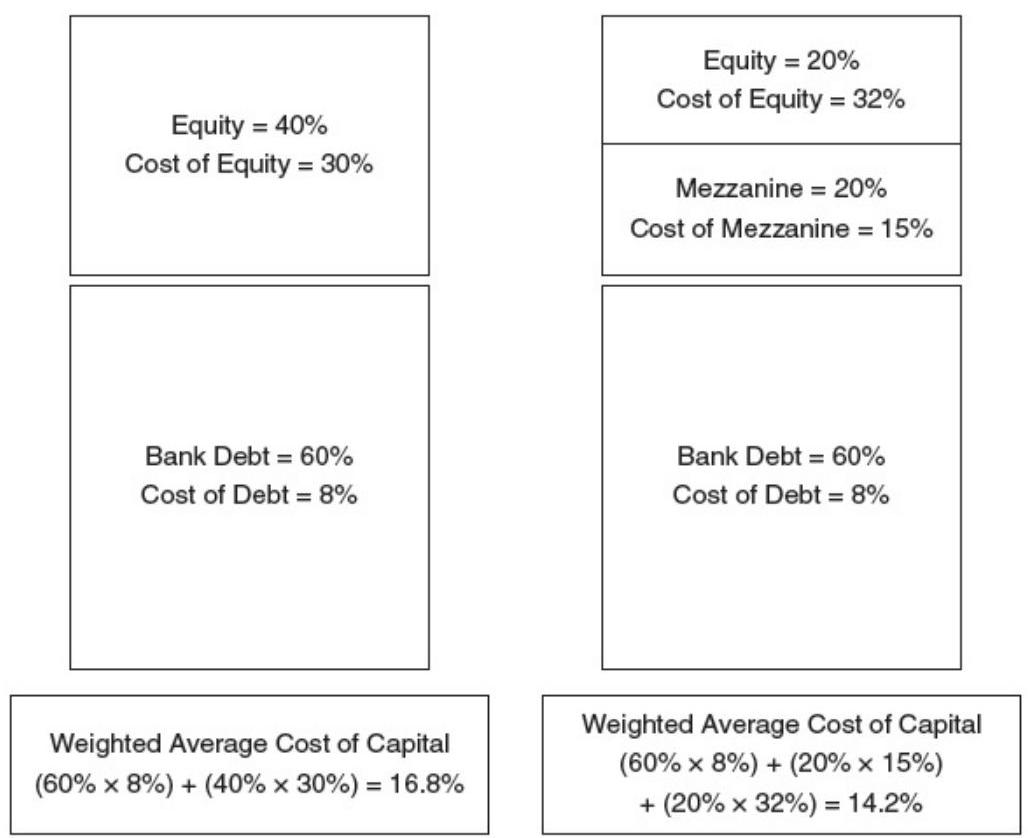
\includegraphics[max width=\textwidth, center]{2024_04_10_62fc48f41306c58a4ec6g-3}

\section*{Mezzanine Financing and the Cost of Capital}
The right-hand side of the above exhibit lays out how mezzanine capital might lower the capital costs for a company. In this example, half of the equity capital is replaced with mezzanine debt at a coupon rate of $15 \%$. This makes the equity riskier and therefore likely to increase its cost of capital, which is assumed to rise to $32 \%$. At the bottom of the exhibit, the new weighted average cost of capital for the company is calculated. When mezzanine debt is added to the capital structure, the WACC declines from $16.8 \%$ to $14.2 \%$.

The reduced weighted average cost of capital is generated by replacing relatively expensive equity financing with less expensive mezzanine financing. The reduction in capital costs illustrated in the above exhibit demonstrates the motivation for a firm to use mezzanine financing.

This simplified example assumes that the required return on equity changes only slightly when half of the equity is replaced with mezzanine debt and the leverage is increased. In the case of very-well-functioning capital markets, it would usually be argued that sources of financing are efficiently priced and that different capital structures cannot be used to generate lower aggregate costs of capital (i.e., lower weighted average costs of capital). The justifications for advantages to mezzanine debt are based on inefficiencies and imperfections in the capital markets for the size of companies that tend to use mezzanine financing.

\section*{Mezzanine Financing Compared with Other Forms of Financing}
Generally, mezzanine financing occurs in amounts below $\$ 400$ million. In other words, mezzanine financing is generally used by middle-market companies, which are the larger stocks within the small-cap classification. These firms do not usually have access to the large public debt markets as a relatively efficiently priced source of debt capital. High-yield debt issues tend to start at sizes of $\$ 400$ million. The same is true for leveraged loans.

Mezzanine financing is highly negotiated and can be tailored to any company's situation. The flip side is that the level of tailoring makes mezzanine debt illiquid. Exiting mezzanine debt involves a lengthy negotiation process for the investor, either with the company that issued the mezzanine debt to buy back its securities or with a secondary private equity investor to purchase the position. In both cases, mezzanine debt is often sold at a large discount.

Mezzanine debt is typically held by mezzanine debt funds raised by private equity firms. Mezzanine financing stands behind senior debt and is usually analyzed on an earnings before interest, taxes, depreciation, and amortization (EBITDA) multiple basis. Bank loans and other senior loans generally require a loan-to-EBITDA multiple of no more than 2 to 2.5 . In other words, a firm with EBITDA of $\$ 100$ million per year would typically be allowed to borrow between $\$ 200$ million and $\$ 250$ million in senior loans. However, mezzanine debt typically allows for a higher loan-to-EBITDA multiple. Thus, with a multiple of 4 to 4.5, a firm with EBITDA of $\$ 100$ million per year could expand its total debt to between $\$ 400$ million and $\$ 450$ million, including perhaps $\$ 225$ million of senior debt and $\$ 200$ million of mezzanine debt. As shown in the next exhibit, debt multiples for buyout transactions have been increasing, with total debt loads now exceeding six times EBITDA.

\begin{center}
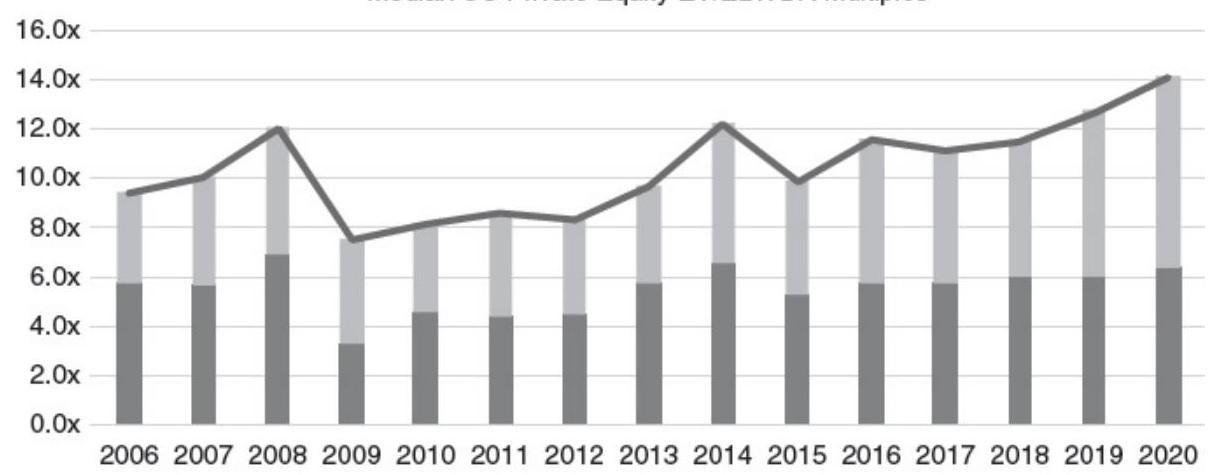
\includegraphics[max width=\textwidth]{2024_04_10_62fc48f41306c58a4ec6g-4}
\end{center}

Debt/EBITDA Equity/EBITDA EV/EBITDA

Deal Multiples and Leverage Multiples Have Been Rising in Large U.S. LBOs

Source: Pitchbook, 2020 Annual US PE Breakdown.

Because mezzanine debt is not backed by collateral, it carries a higher coupon payment than does senior debt. Mezzanine debt is generally medium-term money, usually with maturities from five to seven years. Typically, mezzanine financing requires only payment of interest until maturity; there is no amortization of the underlying debt. Mezzanine debt often includes a payment in kind (PIK) toggle. A PIK toggle allows the underlying company to choose whether it will make required coupon payments in the form of cash or in kind, meaning with more mezzanine bonds. Leveraged loans do not have such a provision.

The next exhibit compares mezzanine debt to leveraged loans and high-yield bonds. Notice that leveraged loans have the strictest debt covenants, which lead to greater protection from default but also to a lower return. Also, a credit rating is typically required before a bank will lend credit through a leveraged loan, whereas this is not necessary for mezzanine debt. In addition, leveraged loans typically have a floating interest rate tied to the London Interbank Offered Rate (LIBOR), whereas mezzanine debt has a fixed coupon.

Comparison of Leveraged Loans, High-Yield Bonds, and Mezzanine Debt

\begin{center}
\begin{tabular}{|l|l|l|l|}
\hline
 & Leveraged Loans & High-Yield Bonds & Mezzanine Debt \\
\hline
Seniority & Most or second-most senior & Contractual and structural subordination & Lowest priority \\
\hline
Type of security & First or second lien on assets & Unsecured & Unsecured \\
\hline
Credit rating & Usually required & Required & Not required \\
\hline
Loan covenants & Extensive & Less comprehensive & Minimal: typically related only to payment of coupons \\
\hline
Term & 5 years & $7-10$ years & $4-6$ years \\
\hline
Amortization & Installments & Bullet payment & Bullet payment \\
\hline
Coupon type & Cash/floating & Cash/fixed & Cash/PIK/fixed \\
\hline
Coupon rate & LIBOR + spread & $5 \%-8 \%$ & $8 \%-11 \%$ \\
\hline
Prepayment penalty & Usually none & High: usually the company must pay a call premium & Moderate: sometimes equity conversion is forced \\
\hline
Equity kicker & None & Sometimes & Almost always: usually equity warrants \\
\hline
Recovery if default & $60 \%-100 \%$ & $40 \%-50 \%$ & $20 \%-30 \%$ \\
\hline
Liquidity & High & Low & Minimal \\
\hline
\end{tabular}
\end{center}

The risk of bonds or loans can be differentiated even further based on whether a transaction is sponsored or unsponsored. Many private credit funds participate in sponsored lending, whereby the borrowing firm is backed by an investment from a private equity fund or buyout fund sponsor. Investing in the debt that's generated through an LBO transaction might be a bit safer because there's a private equity or a buyout fund that owns the equity and maybe some of the debt of the firm. When that firm starts to experience distress, hopefully, the private equity or buyout manager will step in and inject additional capital, which might help to protect the value of their equity investment. A sponsored lending transaction may be therefore less risky than a nonsponsored lending transaction, because a nonsponsored transaction doesn't have that private equity manager who might be willing to come and invest additional equity in the firm when it becomes distressed.

One last point is that leveraged loans do not contain any type of equity kicker, so they do not share in any upside of the company. Mezzanine debt investors focus on the total return from mezzanine financing, including future equity participation through a convertible security or warrants attached to the mezzanine debt. This is distinctly different from bank loans, which focus exclusively on the cash yield. High-yield bonds fall somewhere between these two forms of financing.

\section*{Seven Basic Examples of Mezzanine Financing}
As noted earlier, mezzanine financing can be viewed as filling either a gap in a company's financial structure or a gap in the supply of capital in the financial markets. This makes mezzanine financing extremely flexible. The diversity of transaction types that follow demonstrates this flexibility.

There are seven basic transactions to which mezzanine debt is applied: management buyouts, growth and expansion, acquisitions, recapitalizations, real estate financing, leveraged buyouts, and bridge financing.

\begin{enumerate}
  \item Mezzanine financing for a management buyout (MBO): When the senior management team of a firm leads an MBO, mezzanine debt can fill the gap between senior debt claims and equity.

  \item Mezzanine financing for growth and expansion: A company pursuing growth that cannot raise traditional bank financing or public financing may seek mezzanine financing.

  \item Mezzanine financing for an acquisition: A middle-market company seeking to purchase an even smaller company may seek mezzanine debt financing as part of the capital for the acquisition.

  \item Mezzanine financing to recapitalize a company: Mezzanine debt may be used as part of a new capital structure for a firm to create a new balance sheet, such as having a senior term loan, senior subordinated mezzanine debt, junior subordinated mezzanine debt, convertible preferred stock, and common equity.

  \item Mezzanine financing in commercial real estate: Mezzanine capital fills the gap between first-mortgage financing, which usually has a loan-to-value ratio of $40 \%$ to $75 \%$, and the equity contributed to the project. Typical equity contributions for real estate are in the $10 \%$ to $15 \%$ range. It is in between bank loans and equity that mezzanine financing exists, historically supplying $10 \%$ to $40 \%$ of a project's capital structure.

  \item Mezzanine financing in a leveraged buyout: Mezzanine financing is an established component of many leveraged buyouts. An LBO requires a large amount of debt, and not all debt can be senior. A significant amount of the financing may come from mezzanine investors.

  \item Mezzanine financing as bridge financing: Often, a good portion of the initial debt in an LBO is raised as bridge financing. Bridge financing is a form of gap financing-a method of debt financing that is temporarily used to maintain liquidity while waiting for an anticipated and reasonably expected inflow of cash.

\end{enumerate}

\section*{Investors in Mezzanine Debt}
This section reviews four major types of investors in mezzanine debt:

\begin{enumerate}
  \item Mezzanine funds: Mezzanine funds are organized like hedge funds, venture capital funds, and buyout funds. Investors in mezzanine funds are generally pension funds, endowments, and foundations. These institutional investors do not have the internal infrastructure or expertise to invest directly in the mezzanine market. Therefore, they enter this alternative investment strategy as limited partners through a mezzanine fund.
\end{enumerate}

Mezzanine funds tend to charge a fee structure similar to venture capital (VC) and LBO funds: a management fee in the $1 \%$ to $2 \%$ range and a profit-sharing fee of $20 \%$. Like hedge funds, VC funds, and LBO funds, mezzanine funds are managed by a general partner who has full investment discretion. Many mezzanine funds are managed by merchant banks that have experience with gap financing or by mezzanine professionals who previously worked in the mezzanine departments of insurance companies and banks.

There are two key distinctions between other private equity funds and mezzanine funds. The first lies in return expectations. Mezzanine funds seek total rates of return in the $15 \%$ to $20 \%$ range. Compare this to LBO funds, which seek returns in the $20 \%$ to $30 \%$ range, and VC funds, which seek returns in the $30 \%$ to $50 \%$ range. This puts mezzanine funds at the lower end of the private equity risk-return spectrum. However, contrasted to debt, mezzanine financing is the most expensive because it is the last to be repaid, ranking at the bottom of the creditor spectrum, just above equity. Second, mezzanine fund staff have different expertise than is typically found at a venture capital fund. Most VC funds have staff with heavy technology-related experience, including former senior executives of medical, software, semiconductor, and Internet companies. In contrast, mezzanine funds are inundated with financial engineers who are experienced at structuring and negotiating loans that incorporate the use of equity kickers and warrants.

Mezzanine funds look for businesses that have a high potential for growth and earnings but do not have a sufficient cash flow to receive full funding from banks or other senior creditors. Banks may be unwilling to lend because of a short operating history or a high debt-to-equity ratio. Mezzanine funds look for companies that can repay the mezzanine debt over the next four to seven years through a debt refinancing, an initial equity offering, or being acquired. Mezzanine funds are considerably smaller than the huge ( $\$ 20$ billion plus) leveraged buyout funds. This reflects the fact that mezzanine financing is distinctly a middle-market phenomenon and cannot support megafunds of the type commonly associated with LBOs.

Mezzanine funds are risk lenders. This means that in a liquidation of the company, mezzanine investors expect little or no recovery of their principal. Mezzanine debt is rarely secured. As the last rung of the financing ladder, it is often viewed as a form of equity by the more senior lenders.

\begin{enumerate}
  \setcounter{enumi}{1}
  \item Insurance companies: Insurance companies are a major source of mezzanine financing. They are natural providers of mezzanine debt because the durations of their liabilities (life insurance policies and annuities) are best matched with longer-term debt instruments. These investors take more of a fixed-income approach and place a high value on the scheduled repayment of principal. Insurance companies are more concerned with a higher coupon payment than with the total return, including equity warrants. Therefore, insurance companies act more like traditional lenders than like equity investors. They provide mezzanine financing to higher-quality credit names and emphasize preservation versus appreciation of capital.

  \item Traditional senior lenders: Interestingly, banks and other providers of senior secured debt often participate in mezzanine financing. This financing takes the form of so-called stretch financing, where a bank lends more money than it believes would be prudent with traditional lending standards and traditional lending terms. This excess of debt beyond the collateral value of a company's business assets is the "stretch" part of the financing. Senior lenders may ask for an equity kicker, such as warrants, to compensate the institution for stretching financing beyond the assets available.

  \item Traditional venture capital firms: When the economy softens, venture capital firms look for ways to maintain their stellar returns. In addition, times of large flows of capital into venture capital funds make it necessary for them to expand their investment horizons, resulting in a greater interest in mezzanine financing. Mezzanine financing and venture capital frequently go hand in hand, with mezzanine debt serving as the bridge. In this case, the bridge is the last round of private financing before a start-up company goes public. The lines between mezzanine financing and different forms of private equity can become blurred. With respect to pre-initial public offering (IPO) companies, it is difficult to distinguish where venture capital ends and mezzanine financing begins. Also, mezzanine financing can be used as the last leg in the capital structure of a start-up company before it goes public. This bridge financing allows the company to clean up its balance sheet before its IPO.

\end{enumerate}

\section*{Eight Characteristics of Mezzanine Debt}
Mezzanine debt has eight characteristics that help distinguish it from other sources of financing and types of investments:

\begin{enumerate}
  \item Board representation: A subordinated lender generally expects to be considered an equity partner. In some cases, mezzanine lenders may request board observation rights; in other cases, mezzanine lenders may insist on a seat on the board of directors with full voting rights.

  \item Restrictions on the borrower: Although mezzanine debt is typically unsecured, it may still come with restrictions on the borrower. The mezzanine lender may have the right to approve or disapprove of additional debt and require that any new debt be subordinated to the original mezzanine debt. The lender may also enjoy final approval over any contemplated acquisitions, changes in the management team, or payment of dividends.

  \item Flexibility: There are no set terms to mezzanine financing. The structure of mezzanine debt can be as flexible as needed to accommodate the parties involved. For example, mezzanine debt can be structured so that no interest payments begin for two to three years.

  \item Negotiations with senior creditors: The subordination of mezzanine debt is typically accomplished with an intercreditor agreement. An intercreditor agreement is an agreement with the company's existing creditors that places restrictions on both the senior creditor and the mezzanine investor. The intercreditor agreement may be negotiated separately between the senior creditors and the mezzanine investor, or it may be incorporated directly into the loan agreement between the mezzanine investor and the company. Intercreditor agreements usually restrict amendments to the credit facility so that the terms of the intercreditor agreement cannot be circumvented by new agreements between the individual lenders and the borrower.

  \item Subordination: The subordination (lowered priority) may be either a blanket subordination or a springing subordination. A blanket subordination prevents any payment of principal or interest to the mezzanine investor until after the senior debt has been fully repaid. A springing subordination allows the mezzanine investor to receive interest payments while the senior debt is still outstanding. However, if a default occurs or a covenant is violated, the subordination springs up to stop all payments to the mezzanine investor until either the default is cured or the senior debt has been fully repaid.

  \item Acceleration: The violation of any covenant may result in acceleration. Acceleration is a requirement that debt be repaid sooner than originally scheduled, such as when the senior lender can declare the senior debt due and payable immediately. This typically forces a default and allows the senior lender to enforce the collateral security.

  \item Assignment: Senior lenders typically restrict the rights of the mezzanine investor to assign, or sell, its interests to a third party. However, senior lenders generally allow an assignment, providing the assignee executes a new intercreditor agreement with the senior lender.

  \item Takeout provisions: A takeout provision allows the mezzanine investor to purchase the senior debt once it has been repaid to a specified level. This is one of the most important provisions in an intercreditor agreement and goes to the heart of mezzanine investing. By taking out the senior debt, the mezzanine investor becomes the most senior level of financing in the company and, in fact, can take control of the company. At this point, the mezzanine investor usually converts the debt into equity through either convertible bonds or warrants and becomes the largest shareholder of the company.

\end{enumerate}

\end{document}